\chapter{Workers and Resources}
\label{ch:resources}
This chapter covers the related to gathering resources, and how we handle this with the agent including the worker management architecture. 

In early- and mid-game, \emph{economic advantage} is the most important aspect of StarCraft strategy. This occurs when you have a higher resource intake than your opponent, such as if you have more workers that are gathering or more bases to gather from. The advantage is while maintaining an equivalent army to the opponent, one can replace lost troops faster, gain a larger army or upgrade the current one. If you eclipse your opponent in resources, you can perform worse in combat and still win. Without the advantage, upgrading troops would slow troop production down and the opponent could produce an equivalent or even stronger army at any time.

\begin{figure}
	\centering
	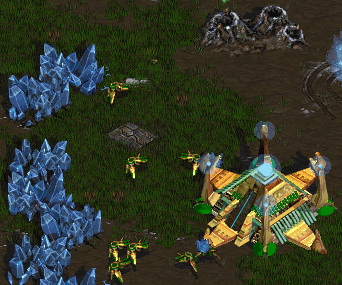
\includegraphics{figures/Resources}
	\caption{A screenshot of resources with minerals on the left and a vespene geyser at the top. The structure to the lower right is a depot.}
	\label{fig:resources}
\end{figure}

There are three kinds resources in StarCraft: \emph{minerals}, \emph{gas} and \emph{supply}. \emph{Workers} are the only units capable of gathering resources. Each race has one worker type and each player start the game with a couple of their race's type. Players also start with a \emph{resource depot} or simply \emph{depot}. This structure can produce new workers and is also the drop off point for gathering resources. The Protoss worker is the \emph{probe} and their depot is the \emph{nexus}. Figure \ref{fig:resources} depicts workers gathering minerals and returning them to the depot.

\emph{Minerals} are mined from mineral fields which usually are in clusters of 8-12. All units cost minerals, so it is the most important resource. Workers that mine these bring them back to the depot in batches of six mineral units. Depot's are limited in their proximity to the clusters, but at optimal distance there can be a maximum of three workers on each field. Mineral fields are usually placed in a half-circle formation, such that there exists an optimal depot location. While the first worker on each mineral field will gather at a linear rate, they will yield diminishing returns on the second and especially third worker.

\emph{Vespene Gas} or simply \emph{gas} is harvested from \emph{refineries}. Each race has a distinct refinery structure, although they are very similar. These must be built upon \emph{Vespene Geysers} of which there are up to two by each mineral cluster. It is harvested in batches of eight with a max of three workers per refinery at optimal depot distance. Advanced structures, units and all technologies depend on gas. The immediate cost of the refinery and lost mineral gathering is a liability against fast openings, but harvesting too late means fighting against stronger units.

The last resource, \emph{supply} is a population limit and is cannot be gathered like the other resources. Each unit reserves some amount of supply which is released upon their destruction. The only way to increase the supply limit is producing the race's supply unit. Each race has exactly one unit which increases the limit by a constant amount per instance, which is subtracted if they are destroyed. Units cannot be produced if they require more supply than the player has free. If the player happens to use more supply than their limit, they will be unable to build more units until more supply is acquired, called \emph{supply blocked}. Although supply is specifically the Terran resource, it is used as the general term for all races. \emph{Psi} and \emph{control} are the Protoss and Zerg equivalents. The Protoss supply unit is the \emph{pylon} structure.

While multiple workers can gather from the same field or refinery, only one worker can actively occupy it. The rest is either returning cargo, moving to the resource or waiting.

In the next sections we will first describe the architecture behind worker management, followed by how minerals is mined and gas is harvested. Building supply is first covered in Chapter \ref{ch:strategy}, as this resources behaves much different than the others.

\section{Managing Workers}
\label{sec:manageWorkers}
The \emph{Task Master} module contains workers related to a single depot. Every depot has its own instance of the module, separating the workers into resource clusters for easy gathering. The task master keeps the workers in sets and also designates a \emph{task} for each worker. Initially a worker is tasked as \texttt{idle}, but other modules could re-task workers, essentially allocating and freeing workers. Each task has a related set of workers, stored as a dictionary of sets. Given $n$ workers and a small amount of tasks, insertions, deletions and re-tasks operations has time complexity $O(\log n)$. We expect $n$ to be in the range of $0-24$, so the operations are quite fast. The current set of tasks are \texttt{idle}, \texttt{mine}, \texttt{harvest}, \texttt{build} and \texttt{defend}.

Every task master is wrapped in a \emph{Vassal} module, all of which are contained in a dictionary within the \emph{Landlord} module. As the amount of needed Vassal instances are unknown, they are stored in dynamic memory. The Landlord designates new workers to or destroyed from the related Vassal. This allows for easier operations from superior modules to the worker pool.

The \emph{Gatherer} module commands all gathering workers, superior only to the Landlord module and its immediate subordinates. Resource gathering was initially kept within each task master, however this makes it difficult to control gathering on a large scale. The resource priorities should not necessarily be uniform across all bases. Each frame, the Gatherer iterates through the vassals, commanding current gatherers and re-tasking all idle workers to gathering. How this is handled is explained the following sections.

\section{Mining Minerals}
StarCraft has a built-in worker gathering AI to help human players. Workers will automatically return cargo from resources (unless they are interrupted) and return to the same resource afterwards. When gathering minerals, they will move to another mineral field if the current one is occupied. This is an inefficient solution, as the worker could be stuck moving between minerals for long periods of time. It is also a liability for a bot, as the AI cannot be disabled. When harvesting gas they will wait until the refinery is unoccupied.

The simplest mineral gathering implementation is ordering idle gatherers to mine some arbitrary mineral. At some point, the built-in AI will ensure the workers are optimally scattered. It will however not be scattered immediately, and some workers will be very inefficient while moving from mineral to mineral. A simple but effective addition would be to scatter the initial workers.

By maintaining a queue of minerals, we can optimally scatter the workers. The first element of the queue is the mineral with fewest workers and the one in the back has the most. By continually assigning new workers to the first element and moving it to the back, we maintain a queue where the last mineral has at most one more worker than the first. Removing workers however requires finding the mineral in the queue, and should be done sparingly. Therefore, it is assumed any building or defending activity will be short and temporary, and workers assigned such will not be removed from the scattering. This might result in an ineffective scattering at some points. It is not clear however if optimizing the scattering at all times results in optimal resource output, as workers might be moved between minerals too often, resulting in less time mining. Figure \ref{fig:minerals} visualizes the worker scattering.

\begin{figure}
	\centering
	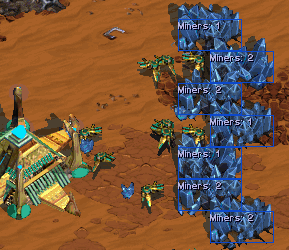
\includegraphics{figures/Minerals}
	\caption{A screenshot of minerals, where each has some assigned miners.}
	\label{fig:minerals}
\end{figure}

If we maintain a dictionary of workers and their targets, we can assign new ones in constant time and retrieving targets in logarithmic time. This could be improved to amortized constant time with hashing. Removing a worker however requires a search through the queue which is linear time.

\section{Harvesting Gas}	
Gas harvest is very much like mineral mining, but simpler. Rarely will players have fewer than three workers on each refinery, as refineries will be built only when needed. Furthermore, almost all late-game units require gas, and harvesting is slower than mining.

The implementation is identical to mineral mining. No AI tournament maps contain more than one refinery, but the gas harvesting still uses a priority queue. In this case however, all operations become constant time, so performance is not harmed while code is reused.